\documentclass[tikz,border=8pt]{standalone}
% Shared look for every TikZ diagram. Load with % Shared look for every TikZ diagram. Load with % Shared look for every TikZ diagram. Load with \input{../../tools/tikz-style.tex}
\usepackage[T1]{fontenc}
\usepackage{lmodern}
\renewcommand{\sfdefault}{lmr}  % diagrams use the same serif as the text
\usetikzlibrary{arrows.meta, positioning, shapes.geometric, calc, fit, backgrounds}
\definecolor{cblue}{HTML}{4C78A8}
\definecolor{corange}{HTML}{F58518}
\definecolor{cgreen}{HTML}{54A24B}
\definecolor{cred}{HTML}{E45756}
\definecolor{cpurple}{HTML}{B279A2}
\definecolor{cgrey}{HTML}{6B6B6B}
\tikzset{
  every picture/.style={font=\sffamily, line width=1.2pt},
  box/.style={draw=#1, fill=#1!12, rounded corners=4pt, align=center, inner sep=7pt, minimum height=1.1cm},
  box/.default=cgrey,
  arrow/.style={-{Stealth[length=3mm]}, draw=cgrey, line width=1.4pt},
  title/.style={font=\sffamily\bfseries\Large},
  note/.style={font=\sffamily\small, text=cgrey, align=center},
}
\AtBeginDocument{\hyphenpenalty=10000 \exhyphenpenalty=10000}

\usepackage[T1]{fontenc}
\usepackage{lmodern}
\renewcommand{\sfdefault}{lmr}  % diagrams use the same serif as the text
\usetikzlibrary{arrows.meta, positioning, shapes.geometric, calc, fit, backgrounds}
\definecolor{cblue}{HTML}{4C78A8}
\definecolor{corange}{HTML}{F58518}
\definecolor{cgreen}{HTML}{54A24B}
\definecolor{cred}{HTML}{E45756}
\definecolor{cpurple}{HTML}{B279A2}
\definecolor{cgrey}{HTML}{6B6B6B}
\tikzset{
  every picture/.style={font=\sffamily, line width=1.2pt},
  box/.style={draw=#1, fill=#1!12, rounded corners=4pt, align=center, inner sep=7pt, minimum height=1.1cm},
  box/.default=cgrey,
  arrow/.style={-{Stealth[length=3mm]}, draw=cgrey, line width=1.4pt},
  title/.style={font=\sffamily\bfseries\Large},
  note/.style={font=\sffamily\small, text=cgrey, align=center},
}
\AtBeginDocument{\hyphenpenalty=10000 \exhyphenpenalty=10000}

\usepackage[T1]{fontenc}
\usepackage{lmodern}
\renewcommand{\sfdefault}{lmr}  % diagrams use the same serif as the text
\usetikzlibrary{arrows.meta, positioning, shapes.geometric, calc, fit, backgrounds}
\definecolor{cblue}{HTML}{4C78A8}
\definecolor{corange}{HTML}{F58518}
\definecolor{cgreen}{HTML}{54A24B}
\definecolor{cred}{HTML}{E45756}
\definecolor{cpurple}{HTML}{B279A2}
\definecolor{cgrey}{HTML}{6B6B6B}
\tikzset{
  every picture/.style={font=\sffamily, line width=1.2pt},
  box/.style={draw=#1, fill=#1!12, rounded corners=4pt, align=center, inner sep=7pt, minimum height=1.1cm},
  box/.default=cgrey,
  arrow/.style={-{Stealth[length=3mm]}, draw=cgrey, line width=1.4pt},
  title/.style={font=\sffamily\bfseries\Large},
  note/.style={font=\sffamily\small, text=cgrey, align=center},
}
\AtBeginDocument{\hyphenpenalty=10000 \exhyphenpenalty=10000}

\begin{document}
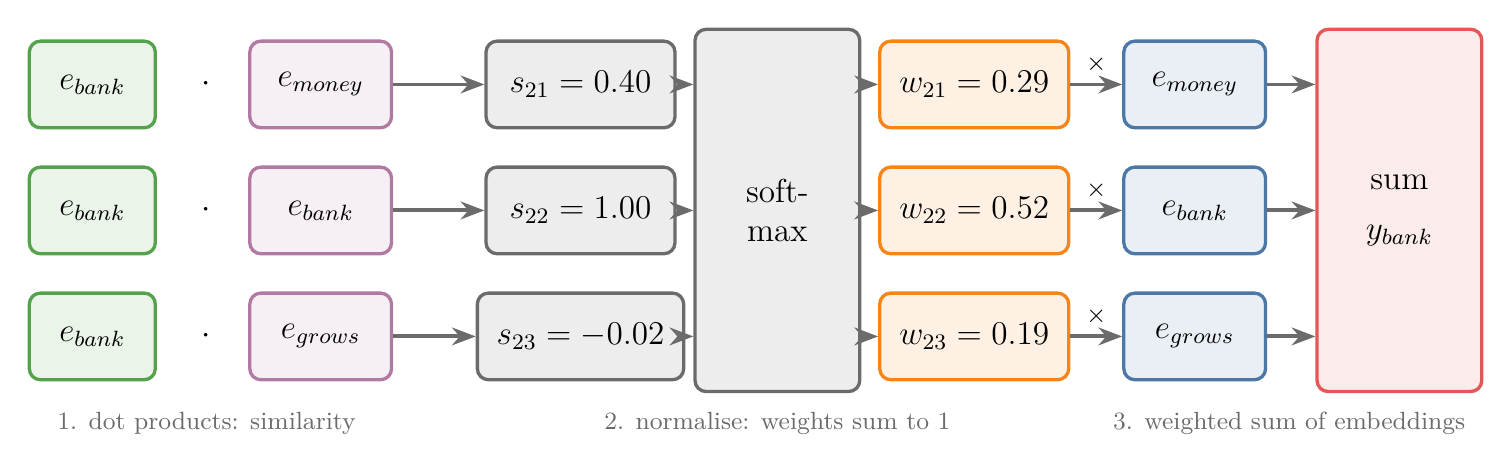
\begin{tikzpicture}[every node/.append style={font=\sffamily\large}]
  \foreach \j/\w/\s/\wt/\y in {1/money/0.40/0.29/1.6, 2/bank/1.00/0.52/0, 3/grows/-0.02/0.19/-1.6} {
    \node[box=cgreen, minimum width=1.6cm] (q\j) at (0,\y) {$e_{\text{bank}}$};
    \node[box=cpurple, minimum width=1.8cm] (k\j) at (2.9,\y) {$e_{\text{\w}}$};
    \node[box=cgrey, minimum width=2.4cm] (s\j) at (6.2,\y) {$s_{2\j} = \s$};
    \node[box=corange, minimum width=2.4cm] (w\j) at (11.2,\y) {$w_{2\j} = \wt$};
    \node[box=cblue, minimum width=1.8cm] (v\j) at (14.0,\y) {$e_{\text{\w}}$};
    \node at ($(q\j)!0.5!(k\j)$) {$\cdot$};
    \draw[arrow] (k\j) -- (s\j);
    \draw[arrow] (w\j) -- node[above, font=\sffamily\small] {$\times$} (v\j);
  }
  \node[box=cgrey, minimum height=4.6cm, text width=1.6cm] (sm) at (8.7,0) {soft-\\max};
  \foreach \j in {1,2,3} {\draw[arrow] (s\j.east) -- (sm.west |- s\j.east); \draw[arrow] (sm.east |- w\j.west) -- (w\j.west);}
  \node[box=cred, minimum height=4.6cm, text width=1.6cm] (sum) at (16.6,0) {sum\\[4pt]$y_{\text{bank}}$};
  \foreach \j in {1,2,3} \draw[arrow] (v\j.east) -- (sum.west |- v\j.east);
  \node[note] at (1.45,-2.7) {1. dot products: similarity};
  \node[note] at (8.7,-2.7) {2. normalise: weights sum to 1};
  \node[note] at (15.2,-2.7) {3. weighted sum of embeddings};
\end{tikzpicture}
\end{document}
